\documentclass[runningheads]{llncs}

% ---------------------------------------------------------------
% Include basic ECCV package
 
% TODO REVIEW: Insert your submission number below by replacing '*****'
% TODO FINAL: Comment out the following line for the camera-ready version
\usepackage[review,year=2026,ID=5523]{eccv}
% TODO FINAL: Un-comment the following line for the camera-ready version
%\usepackage{eccv}

% OPTIONAL: Un-comment the following line for a version which is easier to read
% on small portrait-orientation screens (e.g., mobile phones, or beside other windows)
%\usepackage[mobile]{eccv}


% ---------------------------------------------------------------
% Other packages

% Commonly used abbreviations (\eg, \ie, \etc, \cf, \etal, etc.)
\usepackage{eccvabbrv}

% Include other packages here, before hyperref.
\usepackage{graphicx}
\usepackage{booktabs}

% \usepackage{hyperref}
\usepackage{url}
\usepackage{multirow}
\usepackage{colortbl}
\usepackage{xcolor}
\usepackage{enumitem}
\usepackage[table]{xcolor}

% The "axessiblity" package can be found at: https://ctan.org/pkg/axessibility?lang=en
\usepackage[accsupp]{axessibility}  % Improves PDF readability for those with disabilities.

\newcommand{\lc}[1]{{\color{blue}{$^\textbf{\emph{Long:}}$[#1]}}}

% ---------------------------------------------------------------
% Hyperref package

% It is strongly recommended to use hyperref, especially for the review version.
% Please disable hyperref *only* if you encounter grave issues.
% hyperref with option pagebackref eases the reviewers' job, but should be disabled for the final version.
%
% If you comment hyperref and then uncomment it, you should delete
% main.aux before re-running LaTeX.
% (Or just hit 'q' on the first LaTeX run, let it finish, and you
%  should be clear).

% TODO FINAL: Comment out the following line for the camera-ready version
\usepackage[pagebackref,breaklinks,colorlinks,citecolor=eccvblue]{hyperref}
% TODO FINAL: Un-comment the following line for the camera-ready version
% \usepackage{hyperref}

% Support for ORCID icon
\usepackage{orcidlink}


\begin{document}

% ---------------------------------------------------------------
% TODO REVIEW: Replace with your title
\title{SPAR: Semantic-Pixel Self-Alignment and Adaptive Routing for Unified Multimodal Models} 

% TODO REVIEW: If the paper title is too long for the running head, you can set
% an abbreviated paper title here. If not, comment out.
\titlerunning{Abbreviated paper title}

% TODO FINAL: Replace with your author list. 
% Include the authors' OCRID for the camera-ready version, if at all possible.
\author{First Author\inst{1}\orcidlink{0000-1111-2222-3333} \and
Second Author\inst{2,3}\orcidlink{1111-2222-3333-4444} \and
Third Author\inst{3}\orcidlink{2222--3333-4444-5555}}

% TODO FINAL: Replace with an abbreviated list of authors.
\authorrunning{F.~Author et al.}
% First names are abbreviated in the running head.
% If there are more than two authors, 'et al.' is used.

% TODO FINAL: Replace with your institution list.
\institute{Princeton University, Princeton NJ 08544, USA \and
Springer Heidelberg, Tiergartenstr.~17, 69121 Heidelberg, Germany
\email{lncs@springer.com}\\
\url{http://www.springer.com/gp/computer-science/lncs} \and
ABC Institute, Rupert-Karls-University Heidelberg, Heidelberg, Germany\\
\email{\{abc,lncs\}@uni-heidelberg.de}}

\maketitle


% \begin{abstract}
% Multimodal Large Language Models (MLLMs) have achieved remarkable success in visual understanding but remain constrained in visual generation due to the fundamental feature discrepancy between semantic perception and pixel-level reconstruction. Bridging this gap is challenging: semantic encoders inherently discard high-frequency spatial details crucial for generation, and existing unified models typically rely on rigid, static feature fusion mechanisms. To address these limitations, we propose a novel unified multimodal framework featuring \textbf{S}emantic-\textbf{P}ixel self-Alignment and \textbf{A}daptive \textbf{R}outing (\textbf{SPAR}). First, we introduce an asymmetric dual-stream unified tokenizer that explicitly decouples semantic preservation and pixel reconstruction. A lightweight semantic stream retains discriminative features, while a Transformer-augmented pixel stream recovers fine-grained visual details, merging them into a unified compact latent space. Second, we propose dynamic token routing, enabling each token to aggregate multi-layer MLLM features based on its semantic role adaptively. Finally, we design a self-aligned generation paradigm that leverages the tokenizer itself as an alignment teacher for the diffusion model, eliminating the dependency on external feature networks. Extensive experiments demonstrate that SPAR establishes a new state-of-the-art for unified architectures. It achieves exceptional reconstruction quality and generation capabilities while fully preserving and even enhancing the foundational visual understanding performance.

%   \keywords{Unified Model \and Multimodal Understanding \and Visual Generation}
% \end{abstract}

% \begin{abstract}
% Multimodal Large Language Models (MLLMs) have achieved remarkable success in visual understanding but remain constrained in visual generation due to the fundamental feature discrepancy between semantic perception and pixel-level reconstruction. Bridging this gap faces two major hurdles: semantic encoders inherently discard high-frequency spatial details crucial for generation, and existing unified models suffer from external alignment and rigid feature fusion. To address these limitations, we propose a novel unified multimodal framework featuring \textbf{S}emantic-\textbf{P}ixel self-Alignment and \textbf{A}daptive \textbf{R}outing (\textbf{SPAR}). First, we introduce an asymmetric dual-stream unified tokenizer that explicitly decouples semantic preservation and pixel reconstruction. A lightweight semantic stream anchors discriminative features, while a Transformer-augmented pixel stream recovers fine-grained visual details into a unified compact latent space. Second, we propose a self-aligned generation paradigm that leverages this optimized tokenizer as an internal alignment teacher for the diffusion model, eliminating the dependency on external feature networks. Finally, we introduce Dynamic Token Routing (DTR), enabling each token to adaptively aggregate multi-layer features based on its distinct semantic demands. Extensive experiments demonstrate that SPAR establishes a new state-of-the-art for unified architectures, achieving exceptional generation and reconstruction quality while fully preserving foundational visual understanding capabilities.

% \keywords{Multimodal Unified Model \and Visual Generation}
% \end{abstract}

\begin{abstract}
Multimodal Large Language Models (MLLMs) have achieved remarkable success in visual understanding but remain constrained in visual generation due to the fundamental feature discrepancy between semantic perception and pixel-level reconstruction.
Bridging this gap requires overcoming two core challenges: endowing semantic encoders with high-fidelity reconstruction capabilities, and effectively aligning generative models with semantic spaces without relying on external teachers.
To this end, we propose a novel unified multimodal framework featuring \textbf{S}emantic-\textbf{P}ixel self-alignment and \textbf{A}daptive \textbf{R}outing (\textbf{SPAR}). First, to reconcile semantic perception with pixel-level reconstruction, we introduce an asymmetric dual-stream unified tokenizer. A lightweight semantic stream anchors discriminative features, while a Transformer-augmented pixel stream recovers fine-grained visual details into a unified compact latent space. Second, to eliminate external dependencies, we propose a self-aligned generation paradigm that natively leverages this optimized tokenizer as an internal alignment teacher for the diffusion model. Furthermore, to facilitate flexible multimodal interaction within this unified space, we introduce Dynamic Token Routing, which enables each token to adaptively aggregate multi-layer MLLM features based on its distinct semantic demands. Extensive experiments demonstrate that SPAR establishes the state-of-the-art for unified architectures, achieving exceptional generation and reconstruction quality while preserving foundational visual understanding capabilities.

\keywords{Unified Model \and Visual Generation \and Visual Tokenizer}
\end{abstract}

\section{Introduction}
Multimodal Large Language Models (MLLMs)~\cite{Qwen3-VL,wang2025internvl3_5,liu2023visual} have demonstrated exceptional performance across a wide range of perception tasks, such as image captioning, visual question answering, and multimodal reasoning, by aligning powerful visual semantic encoders with Large Language Models (LLMs)~\cite{touvron2023llama,qwen3}. 
While these models have become pervasive paradigms in the understanding domain, they have yet to dominate the field of visual generation.
Meanwhile, current state-of-the-art image generation systems~\cite{labs2025flux1kontextflowmatching, flux-2-2025} still rely primarily on low-level, compact latent spaces constructed by Variational Auto-Encoders (VAEs)~\cite{vae}, upon which diffusion processes~\cite{esser2024scaling,rombach2022high} or autoregressive modeling~\cite{TiTok, VAR} are performed.
This leads to a discrepancy in feature patterns between perception and generation models.

\begin{figure}[t]
    \centering
    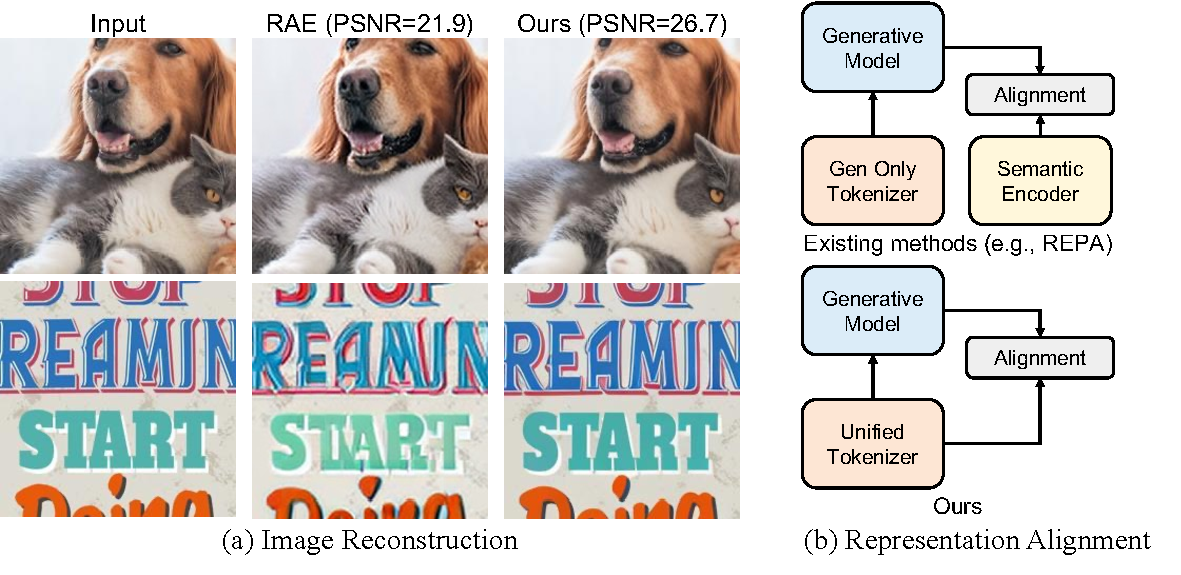
\includegraphics[width=1.\columnwidth]{./images/intro.pdf}
    \vspace{-20pt}
    \caption{\textbf{(a) Image Reconstruction:} When modeling directly within the semantic representation space, existing methods suffer from lossy compression and struggle to preserve high-frequency details. In contrast, our method effectively recovers these crucial pixel-level details. \textbf{(b) Representation Alignment Paradigm:} Unlike existing approaches that rely on external {semantic encoders} to guide the generative model, our framework natively employs the unified tokenizer itself as an alignment teacher.}
    \label{fig:intro}
\end{figure}


Recent studies~\cite{yu2025repa,va-vae,rae} have explored incorporating structured semantic representations (\eg, DINOv2~\cite{oquab2023dinov2}) into generative models. By either aligning diffusion processes with these rich semantic priors or developing generative models directly upon them, these approaches have yielded significant gains in generation quality and convergence speed. 
% The growing efficacy of these semantic spaces in generation reveals a \textcolor{red}{promising convergence point between visual perception and synthesis}. 
The growing efficacy of these semantic spaces in generation reveals a promising path toward unifying visual perception and generation.
This raises \textbf{a natural and critical question}: \emph{Rather than relying on latent spaces, can we seamlessly empower powerful MLLMs with image generation capabilities by shifting the generative modeling space directly to the semantic representation space?} 
% Achieving this would establish a unified multimodal model, intrinsically bridging the gap between understanding and generation.

% However, realizing this paradigm migration is far from straightforward, as an inherent contradiction within the unified tokenizer needs to be overcome.
% Semantic encoders optimized through representation learning have feature spaces that are highly converged toward discriminative tasks.
% This process is essentially a lossy compression of the input image, which tends to discard texture and structural details that are irrelevant to perception but crucial for pixel reconstruction.
% \textcolor{red}{Although RAE~\cite{rae} has successfully implemented a diffusion model within the representation space by the frozen representation encoder while redesigning the Diffusion Transformers (DiTs) to accommodate its high-dimensional semantic feature space, it exhibits significant performance limitations when {scaled to text-to-image generation} and complex instruction-based image editing.}
% This indicates that when directly employing the semantic feature space for generation, the inherently weak reconstruction capability of semantic encoders severely hinders the model's ability to synthesize fine-grained visual information.
% \textcolor{red}{Therefore, how to endow the semantic encoder with high-quality pixel reconstruction capability without compromising its original understanding ability remains the core bottleneck for migrating the generative modeling space to the semantic representation space.} \lc{it would be better to have a figure to demonstrate the weakness of existing method}


% However, realizing this paradigm migration is far from straightforward, as an \textcolor{red}{inherent contradiction within the unified tokenizer} needs to be overcome.
However, realizing this paradigm migration is far from straightforward, as an inherent contradiction between semantic perception and pixel reconstruction needs to be overcome.
Although recent approaches~\cite{rae,va-vae} have successfully implemented diffusion models directly within the semantic representation space, they suffer from severe limitations in image reconstruction quality.
As illustrated in Figure~\ref{fig:intro}(a), RAE~\cite{rae} struggles to preserve high-frequency details, often yielding blurry artifacts and distorted structures.
This occurs because semantic encoders optimized through representation learning have feature spaces that are highly converged toward discriminative tasks. This process is essentially a lossy compression of the input image, which tends to discard texture and structural details that are irrelevant to perception. But these details may be crucial for pixel reconstruction. 
Consequently, this inherently weak reconstruction capability severely hinders the model's synthesis quality when scaled to text-to-image generation and complex instruction-based image editing~\cite{psvae}.
Furthermore, completely fine-tuning the semantic encoder to recover these lost pixel-level details would inevitably trigger catastrophic forgetting, destroying its original understanding abilities.
Therefore, {\emph{how to endow the semantic encoder with high-quality pixel reconstruction capability without compromising its original understanding ability}} remains the core bottleneck for migrating the generative modeling space to the semantic representation space.

% Moreover, an equally critical challenge arises when transmitting multimodal representations from the MLLM to the diffusion model during unified model training. 
% On one hand, although aligning diffusion models with external visual representations~\cite{oquab2023dinov2} has been shown to improve generation quality~\cite{yu2025repa}, recent research~\cite{flux2-vae} indicates that as data scale grows, such forced external alignment is not necessarily the optimal strategy. Consequently, there is an urgent need for an alternative approach that natively aligns the generative process with the MLLM's internal semantic space, eliminating the dependency on external representation learners.
% {On the other hand}, existing unified models exhibit pervasive rigidity in feature fusion: they typically extract only the last layer hidden states of the MLLM.
% This completely ignores that the different tokens have differentiated demands on the model's hierarchical features. For instance, tokens responsible for rendering fine-grained textures require more guidance from low-level structural features, while those responsible for parsing complex instructions are highly dependent on high-level semantic features. 
% % \lc{cannot understand the relation between this challenge and the ``structured semantic representations'' mentioned in the first paragraph.}

Moreover, another critical challenge arises when effectively aligning representations to the generative model during unified model training.
As shown in Figure~\ref{fig:intro}(b), existing representation-aligned generation methods~\cite{yu2025repa,va-vae} typically bridge this gap by enforcing the diffusion model to align with external visual encoders~\cite{oquab2023dinov2} While this forced external alignment provides structured guidance, recent studies~\cite{flux2-vae} suggest that as data scale grows, relying on an isolated external teacher becomes sub-optimal. It risks manifold mismatches between the multimodal understanding and visual generation spaces. Consequently, {\emph{how to natively align the generative model directly with the unified semantic space, and eliminate the dependency on external representation learners}} is a key challenge for effectively training unified understanding and generation models.
% there is an urgent need for a self-alignment framework that

% To address the above challenges, we propose Semantic-Pixel self-alignment and Adaptive Routing (SPAR) for unified multimodal models. \lc{suggestion}
% We introduce an asymmetric dual-stream self-alignment architecture into the unified tokenizer. 
% \textcolor{red}{The lightweight semantic stream preserves the encoder's original discriminative features with minimal transformation cost, while the pixel stream with Transformer augmentation learns to transfer the high-dimensional semantic feature space into the compact pixel latent space of the pixel decoder, thereby recovering the spatial textures and high-frequency details discarded by the encoder's lossy compression.}
% The two streams are fused in a compact latent space, decoupling semantic preservation from pixel reconstruction.
% Notably, the dual-stream-optimized tokenizer itself can serve as the representation alignment teacher for the diffusion model, seamlessly transferring the accumulated semantic and pixel knowledge to the generation stage without relying on any external feature model.
% \textcolor{red}{In addition, to move beyond static feature fusion, we introduce Dynamic Token Routing (DTR), which allows each token to adaptively aggregate multi-layer MLLM features based on its specific semantic role, replacing conventional rigid static extraction.}

To address the above challenges, we propose Semantic-Pixel self-alignment and Adaptive Routing (\textbf{SPAR}) for unified multimodal models. 
To overcome the inherent contradiction between semantic perception and pixel reconstruction, we introduce an asymmetric dual-stream self-alignment architecture into the unified tokenizer. 
The lightweight semantic stream acts as an anchor to preserve the encoder's original discriminative features, preventing catastrophic forgetting. Concurrently, the Transformer-augmented pixel stream is dedicated to mapping the high-dimensional semantic space into a compact latent space, effectively recovering the high-frequency spatial textures discarded by the encoder's lossy compression.
The two streams are fused in a compact latent space, explicitly decoupling semantic preservation from pixel reconstruction. 
Notably, the dual-stream-optimized tokenizer itself can serve as the representation alignment teacher for the diffusion model, seamlessly transferring the accumulated semantic and pixel knowledge to the generation stage without relying on any disjointed external feature model. 
Furthermore, we introduce Dynamic Token Routing (DTR) to facilitate flexible multimodal interaction within this unified space. It empowers each token to adaptively aggregate multi-layer MLLM features based on its distinct semantic role, dynamically satisfying the differentiated hierarchical feature demands of varying tokens.

In summary, our contributions are threefold:
\vspace{-5pt}
\begin{itemize}
    \item We propose a semantic-pixel dual-stream self-alignment architecture that explicitly decouples semantic preservation and pixel reconstruction through an asymmetric design, achieving high-fidelity reconstruction without degrading the encoder's understanding capability.
    \item We introduce dynamic token routing, which enables each token to adaptively determine its own multi-layer fusion weights from the MLLM to optimally harness multimodal representations for generative guidance.
    \item We present a self-alignment generation paradigm that leverages the unified tokenizer as an alignment teacher, removing the dependency on external feature models while achieving competitive results across multiple benchmarks.
\end{itemize}

% To address the aforementioned challenges, we propose Semantic-Pixel self-alignment and Adaptive Routing (SPAR) for unified multimodal models. Specifically, we introduce an asymmetric dual-stream architecture into the unified tokenizer. A lightweight semantic stream preserves the encoder's discriminative features, while a Transformer-augmented pixel stream transfers the high-dimensional semantic space into a compact latent space, effectively recovering the fine-grained details discarded by the encoder's lossy compression. Furthermore, this dual-stream tokenizer naturally serves as the representation alignment teacher for the diffusion model, seamlessly transferring semantic and pixel knowledge to the generation stage without relying on disjointed external models. In addition, to move beyond static feature fusion, we introduce Dynamic Token Routing (DTR), which allows each token to adaptively aggregate multi-layer MLLM features based on its specific semantic role, replacing conventional rigid static extraction.

% In summary, our contributions are threefold:
% \begin{itemize}
% \item We propose an asymmetric semantic-pixel dual-stream tokenizer that explicitly decouples semantic preservation and pixel reconstruction, achieving high-fidelity generation without degrading the encoder's original understanding capability.
% \item We present a self-alignment generation paradigm that leverages the unified tokenizer as an internal alignment teacher. This eliminates the dependency on external feature models and avoids potential manifold mismatches, achieving competitive generation results across multiple benchmarks.
% \item We introduce dynamic token routing, enabling each token to adaptively determine its own multi-layer fusion weights from the MLLM. This mechanism effectively replaces rigid static feature extraction, dynamically satisfying the differentiated hierarchical feature demands of different tokens.
% \end{itemize}

\section{Related Work}

\noindent\textbf{Unified Visual Tokenizer.}
Early approaches~\cite{van2017neural,zhou2024transfusion} relied on reconstruction-focused generative models, which often lack the high-level semantics required for understanding tasks. To address this, recent works have explored unified tokenizers from various perspectives. Some attempt to discretize semantic features directly~\cite{wu2024vila,qu2025tokenflow,ma2025unitok}, but suffer from information loss inherent in quantization. Another recent methods~\cite{tang2025unilip,yue2025uniflow,sun2024generative,svg,rae} attempt to endow pre-trained semantic encoders with pixel reconstruction capabilities via self-distillation and continuous feature alignment. However, forcing a single representation stream to simultaneously accommodate abstract semantics and fine-grained spatial details inevitably leads to capacity bottlenecks and implicit performance trade-offs. To resolve this tension, we explicitly decouple these competing objectives through an unified tokenizer, coordinating visual understanding and generation.

\noindent\textbf{Representation-Guided Generation.}
Pre-trained visual representations are increasingly integrated into diffusion models to enhance semantic and structural fidelity. Recent methods typically achieve this by either explicitly aligning the generative latent space with external discriminative features~\cite{oquab2023dinov2,yu2025repa}, or directly performing diffusion modeling within the semantic space~\cite{rae}. However, these approaches face inherent limitations. As highly abstract semantic spaces naturally discard pixel details, such models often suffer from degraded reconstruction quality and off-manifold artifacts~\cite{psvae}.
% Furthermore, relying on disjointed external teachers introduces system complexity and potential manifold mismatches between the discriminative and generative spaces.
Furthermore, extracting guidance features from external networks forces the generative process to rely on a representation space that is entirely isolated from the model's native visual encoder.
To address this, we introduce a self-aligned generation paradigm. By natively utilizing our explicitly decoupled tokenizer as an internal alignment objective.

\noindent\textbf{Unified Multimodal Understanding and Generation.}
The integration of visual understanding and generation within a single LLM has garnered significant attention. Early unified models~\cite{team2024chameleon, yu2024cm3leon} typically formulated both tasks as next-token prediction within a purely autoregressive framework. To leverage the superior synthesis quality of diffusion models, recent approaches propose attaching diffusion modules directly to the LLM backbone~\cite{sun2023emu, xie2024showo}. To bridge the modality gap, these architectures employ various connection mechanisms. For instance, some methods utilize learnable Q-Formers or linear projectors to align representations~\cite{chen2025blip3, wu2025openuni}, while others adopt Mixture-of-Experts (MoE) or specialized visual queries to manage task routing~\cite{deng2025bagel, tang2025unilip, lin2025uniworld}. 
Despite diverse connector designs, a commonality among these models is their reliance on static, token-agnostic feature extraction (\eg, using only the final layer or fixed fusion weights). This rigid paradigm fails to fully exploit the rich hierarchical representations within MLLMs. To address this, SPAR introduces dynamic token routing to adaptively aggregate multi-layer features for optimal generative guidance.


% \begin{table}[]
% \centering
% \small
% \caption{Comparison with state-of-the-arts on visual understanding benchmarks.}
% \setlength{\tabcolsep}{1pt} % 略微缩小列间距以适应页面宽度
% \begin{tabular}{cccccccccccc}
% \hline
% \multirow{2}{*}{Model} & \multirow{2}{*}{LLM Params} & \multicolumn{3}{c}{Image Reconstruction} & \multicolumn{7}{c}{Image Understanding} \\
%  &  & rFID $\downarrow$ & PSNR $\uparrow$ & SSIM $\uparrow$ & MME-P & MMB & MMMU & MM-Vet & SEED & AI2D & MMVP \\ \hline
% Und. Only &  &  &  &  &  &  &  &  &  &  &  \\
% LLaVA-OV & 1B &  &  &  & 1238 & 52.1 & 31.4 & 29.1 & 65.5 & 57.1 & - \\
% InternVL2.5 & 1B &  &  &  & - & 70.7 & 41.2 & 48.8 & - & 69.3 & 31.3 \\
% InternVL3 & 1B &  &  &  & 1492 & 72.6 & 43.4 & 59.5 & 71.1 & 69.4 & 67.3 \\
% InternVL2.5 & 1.8B &  &  &  & - & 74.7 & 43.6 & 60.8 & - & 74.9 & - \\
% InternVL3 & 1.8B &  &  &  & 1633 & 80.6 & 48.2 & 62.2 & 75.0 & 78.5 & 72.7 \\
% Qwen2.5-VL & 3B &  &  &  & - & 79.1 & 53.1 & 61.8 & - & 81.6 & - \\
% Emu3-Chat & 8B &  &  &  & 1244 & 58.5 & 31.6 & 37.2 & 68.2 & 70.0 & 36.6 \\ \hline
% Gen. Only &  &  &  &  &  &  &  &  &  &  &  \\ \hline
% SD-VAE &  & 2.64 & 22.13 & 0.590 &  &  &  &  &  &  &  \\ \hline
% Und. and Gen. &  &  &  &  &  &  &  &  &  &  &  \\ \hline
% Chameleon & 7B &  &  &  & - & 35.7 & 28.4 & 8.3 & - & - & 0.0 \\
% VILA-U & 7B &  &  &  & 1336 & 66.6 & 32.2 & 27.7 & 56.3 & - & 22.0 \\
% MetaMorph & 8B &  &  &  & - & 75.2 & 41.8 & - & - & - & 48.3 \\
% SEED-X & 13B &  &  &  & 1457 & 70.1 & 35.6 & 43.0 & 66.5 & - & - \\
% TokenFlow-B & 13B &  &  &  & 1354 & 55.3 & 34.2 & 22.4 & 60.4 & 54.2 & - \\
% Show-O & 1.3B &  &  &  & 1097 & - & 26.7 & - & - & - & - \\
% ILLUME & 7B &  &  &  & 1445 & 75.1 & 38.2 & 37.0 & - & 71.4 & - \\
% Janus-Pro & 7B &  &  &  & 1567 & 79.2 & 41.0 & 50.0 & 72.1 & - & - \\
% Harmon & 1.5B &  &  &  & 1155 & 65.5 & 38.9 & - & 67.1 & - & - \\
% MetaQuery-B & 1B &  &  &  & 1238 & 58.5 & 31.4 & 29.1 & 66.6 & - & - \\
% BAGEL & 3B &  &  &  & 1610 & 79.2 & 43.2 & 48.2 & - & - & 54.7 \\
% BLIP3-o & 4B &  &  &  & 1528 & 78.6 & 46.6 & 60.1 & 73.8 & - & - \\
% TokLIP & 7B &  &  &  & 1410 & - & 42.1 & - & 65.2 & - & - \\
% Tar & 7B &  &  &  & 1571 & 74.4 & 39.0 & - & 73.0 & - & - \\
% UniLIP-1B & 1B &  &  &  & 1499 & 72.6 & 43.3 & 59.4 & 71.0 & 70.7 & 68.7 \\
% UniLIP-3B & 2B &  &  &  & 1636 & 80.7 & 48.7 & 62.2 & 75.0 & 78.6 & 73.0 \\ \hline
% SPAR & 1B &  &  &  &  &  &  &  &  &  &  \\ \hline
% \end{tabular}
% \end{table}

\section{Method}
\subsection{Semantic-Pixel Self-Aligned Unified Tokenizer}
% \textcolor{red}{The unified tokenizer aims to construct a visual encoding space that simultaneously preserves discriminative semantic information and pixel-level reconstruction capability, allowing it serve as the visual encoder of the MLLM for understanding tasks while also providing compact latent space for diffusion modeling.}
The unified tokenizer aims to construct a visual encoding space that preserves both discriminative semantic information and pixel-level reconstruction capability. Consequently, it can serve as the visual encoder of the MLLM for understanding tasks while simultaneously providing a compact latent space for diffusion modeling.
% However, the feature space of semantic encoders is heavily biased toward discriminative tasks and is essentially a lossy compression of the input image, discarding high-frequency spatial details irrelevant to semantic classification but crucial for pixel reconstruction.
Training pixel decoders directly on the frozen semantic encoder only yields blurry reconstruction results, while unlocking the encoder for reconstruction training triggers catastrophic forgetting.

\begin{figure}[t]
    \centering
    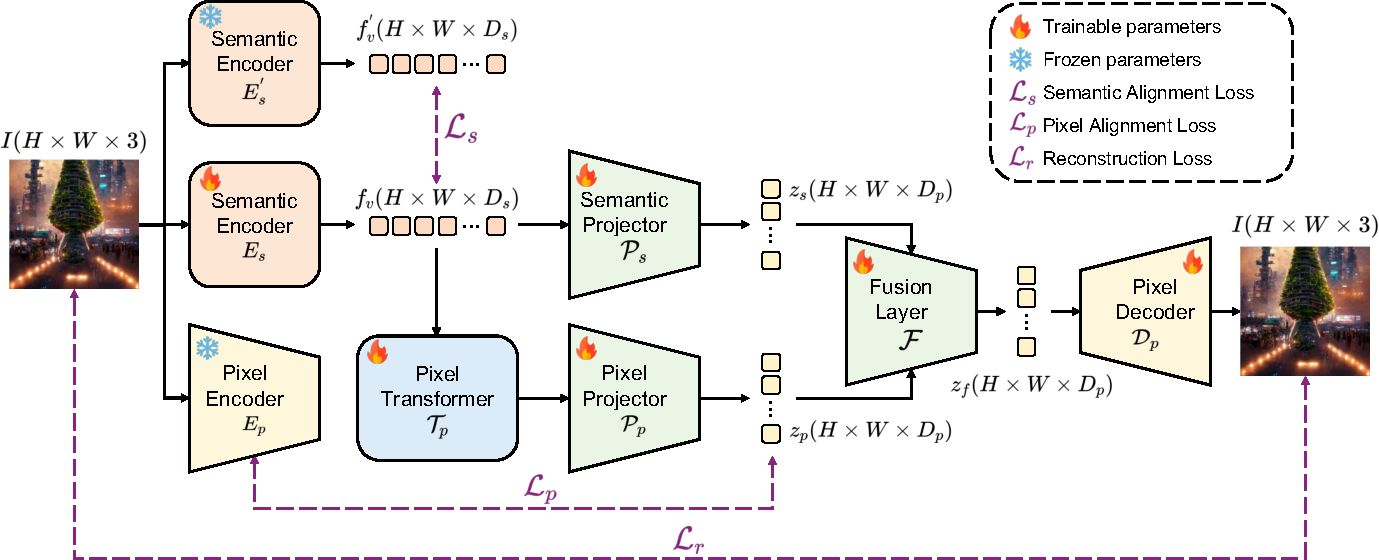
\includegraphics[width=1.\columnwidth]{./images/tokenizer.pdf}
    % \caption{Overview of unified tokenizer.}
    \vspace{-15pt}
    \caption{\textbf{Architecture of the semantic-pixel self-aligned unified tokenizer.}
    Our tokenizer design explicitly decouples semantic preservation from pixel reconstruction.
    A lightweight semantic stream maps features into a compact latent space, strictly anchored by the frozen encoder to prevent catastrophic forgetting ($\mathcal{L}_{s}$). Concurrently, a Transformer-augmented pixel stream bridges the dimensional gap by aligning with the native pixel latent space ($\mathcal{L}_{p}$) to recover high-frequency spatial details. Both streams are fused and decoded to reconstruct the image ($\mathcal{L}_{r}$), endowing the model with high-fidelity generation capabilities without compromising its discriminative understanding.
    }
    \label{fig:tokenizer}
\end{figure}

Semantic information has already been sufficiently encoded in the output features of the pre-trained encoder, and applying excessive transformations would instead perturb the original feature distribution. In contrast, the pixel-level details discarded by the encoder during representation learning require additional computational capacity for recovery. 
Based on this asymmetry, we explicitly decouple the two competing objectives of semantic preservation and pixel reconstruction as shown in~\cref{fig:tokenizer}. 
For the input image $I \in \mathbb{R} ^{H \times W \times 3}$, we construct two different streams on top of the encoder output feature $f_v =E_s(I) \in \mathbb{R}^{H^{'} \times W^{'} \times D_s}$, where $E_s$ is semantic encoder and $D_s$ is the  feature dimension.

\noindent\textbf{Semantic Stream.}
The semantic stream employs a lightweight projector $\mathcal{P}_s$ consisting of multiple residual blocks and an MLP projection layer, which maps the encoder features to the compact latent space with minimal transformation:
$\mathbf{z}_{\text{s}} = \mathcal{P}_s(f_v) \in \mathbb{R}^{H^{'} \times W^{'} \times D_p},$
where $D_p \ll D_s$ is the latent space dimension.
The residual connections ensures the output of the semantic stream to preserve the original discriminative structure of $f_v$ as much as possible, serving as an anchor for the encoder's semantic features in the latent space.

\noindent\textbf{Pixel Stream.}
% \textcolor{red}{A fundamental gap exists between the feature space of the semantic encoder and the compact latent space operated on by the pixel decoder: the former is high-dimensional ($D_s$) and optimized for discriminative objectives, while the latter is low-dimensional ($D_p \ll D_s$) and optimized for pixel reconstruction.}
A fundamental gap exists between the feature space of the semantic encoder and the compact latent space operated on by the pixel decoder. The semantic space is high-dimensional ($D_s$) and optimized for discriminative objectives, whereas the pixel latent space is low-dimensional ($D_p \ll D_s$) and tailored for reconstruction.
For the semantic encoder's output to be correctly decoded by the pixel decoder, an effective mapping from the semantic feature space to the pixel latent space must first be established. The pixel stream is designed as a learnable bridge for this purpose.
It transfers high-dimensional semantic features into the compact pixel latent space, thus allowing the fine-grained details discarded by the encoder during representation learning to be recovered within the pixel decoder's native space.
Specifically, the pixel stream is equipped with an independent Transformer encoder $\mathcal{T}_p$, which models long-range dependencies along the spatial dimension through global self-attention and transforms the semantic features into intermediate representations suitable for pixel reconstruction:
$$f_p = \mathcal{T}_p(f_v) \in \mathbb{R}^{H^{'} \times W^{'} \times D_s}.$$
The Transformer output $f_p$ is then mapped to a compact latent space compatible with the pixel decoder through residual blocks and an MLP projection layer:
$$\mathbf{z}_{\text{p}} = \mathcal{P}_p(f_p) \in \mathbb{R}^{H^{'} \times W^{'} \times D_p}.$$

\noindent\textbf{Fusion \& Decoding}.
The compact latent variables produced by the two streams are merged into a unified representation in the fusion layer $\mathcal{F}$. The semantic latent $\mathbf{z}_{\text{s}}$ and the pixel latent $\mathbf{z}_{\text{p}}$ are concatenated along the channel dimension and then mapped back to the latent space dimension by the fusion layer:
$$\mathbf{z}_f = \mathcal{F}\big([\mathbf{z}_{\text{s}};\, \mathbf{z}_{\text{p}}]\big) \in \mathbb{R}^{H^{'} \times W^{'} \times D_p},$$
where $[\cdot;\cdot]$ denotes channel concatenation. The fused $\mathbf{z}_f$ is fed into the pre-trained pixel decoder $\mathcal{D}_p$ for image reconstruction. This design allows semantic and pixel information to evolve along their respective independent optimization paths before converging in the compact latent space.

\subsection{Progressive Three-Stage Training for Unified Tokenizer}

The training of the unified tokenizer follows a progressive three-stage strategy that gradually releases model capacity, with targeted alignment losses introduced at each stage to guide the optimization direction.

\noindent\textbf{Stage I: Dual-Stream Initialization.}
The vision encoder and pixel decoder are frozen, and only the dual-stream modules are trained. The core objective of this stage is to enable the pixel stream to learn the transfer mapping from the semantic feature space to the pixel latent space. However, the semantic feature space and the pixel decoder's latent space differ fundamentally in dimensionality, distribution, and optimization objectives, making it difficult for the pixel stream to discover the correct mapping direction without explicit supervision. To this end, we introduce the \textbf{pixel alignment loss} that uses the output $\mathbf{z}'_p = E^{'}_p(I)$ of the frozen pixel encoder $E_p$ as an explicit optimization anchor and aligns the pixel stream's latent variables with it:
$$\mathcal{L}_{p} = \| \mathbf{z}_{p} - \mathbf{z}_p^{'} \|_2^2.$$
This loss first guides the pixel stream to transfer the semantic feature space onto the latent manifold of the pixel encoder, aligning its output distribution with the pixel decoder's native encoding. On this basis, the pixel stream can then effectively recover the pixel-level details discarded by the semantic encoder's lossy compression within that space. The complete training loss for this stage is:
$$\mathcal{L}_{\text{I}} = \mathcal{L}_{\text{MSE}} + \mathcal{L}_{\text{LPIPS}} + \lambda_p \mathcal{L}_{p},$$
where $\mathcal{L}_{\text{MSE}}$ represents pixel-wise reconstruction loss, and $\mathcal{L}_{\text{LPIPS}}$ represents the perceptual loss
computed using the LPIPS metric.

\noindent\textbf{Stage II: Joint Decoder Training.} The vision encoder remains frozen while the pixel decoder $\mathcal{D}_p$ is unfrozen for joint training. Only pixel reconstruction losses are used in this stage:
$$\mathcal{L}_{\text{II}} = \mathcal{L}_{\text{MSE}} + \mathcal{L}_{\text{LPIPS}}.$$
The decoder adapts to the latent distribution produced by the dual-stream fusion, maximizing reconstruction quality with a fixed encoder.

\noindent\textbf{Stage III: Encoder Fine-Tuning with Self-Distillation.}
The vision encoder is unfrozen for end-to-end training to further enhance pixel representation capability. However, unfreezing the encoder risks catastrophic forgetting: the gradients from reconstruction training may corrupt the discriminative semantic features accumulated during contrastive learning. To address this, we introduce a \textbf{semantic alignment loss} that uses the features $f'_v=E^{'}_s(I)$ of a frozen encoder to constrain the fine-tuned encoder features to maintain semantic consistency:
$$\mathcal{L}_{s} = \| f_v - f'_v \|_2^2.$$
The encoder learning rate is simultaneously decayed to $0.1\times$ the global learning rate, working together with $\mathcal{L}_{s}$ to form a dual constraint that ensures the encoder does not lose its original semantic understanding performance while acquiring stronger pixel representation capability. Additionally, a GAN discriminator is activated after a certain number of training steps to enhance the perceptual quality of reconstructed images. The complete training loss for this stage is:
$$\mathcal{L}_{\text{III}} = \mathcal{L}_{\text{MSE}} + \mathcal{L}_{\text{LPIPS}} + \lambda_s \mathcal{L}_{s} + \lambda_{\text{GAN}} \mathcal{L}_{\text{GAN}.}$$

\begin{figure}[t]
    \centering
    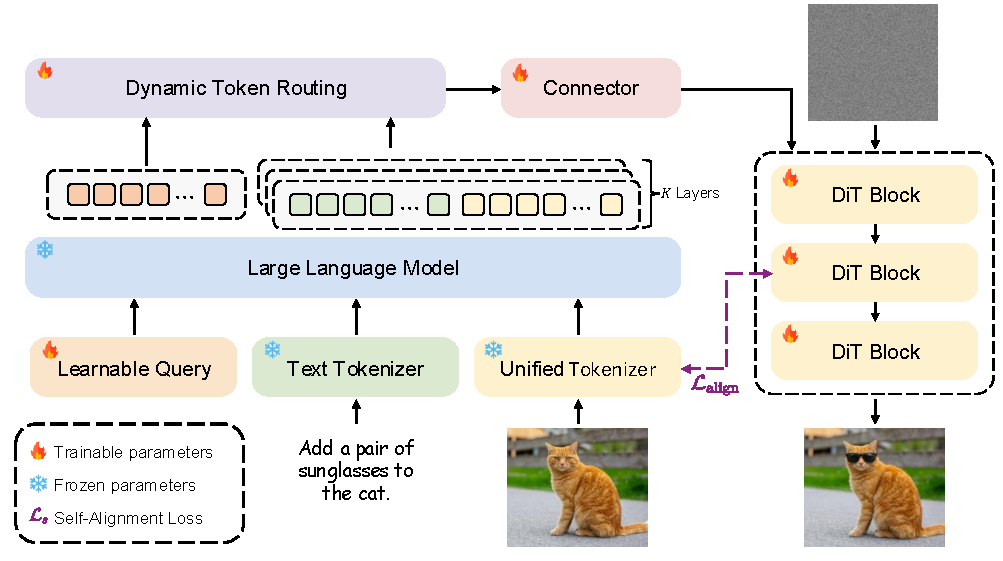
\includegraphics[width=1.\columnwidth]{./images/unified_model.pdf}
    \vspace{-15pt}
    % \caption{Overview of unified model.}
    % \caption{\textbf{Overview of the SPAR Unified Multimodal Model.}
    % The frozen MLLM processes textual instructions, visual references, and learnable queries. To move beyond rigid static feature extraction, our DTR mechanism adaptively aggregates multi-layer MLLM hidden states based on the distinct semantic demands of each token. The fused representations then condition the DiT via a connector. Furthermore, the dual-stream-optimized unified tokenizer naturally serves as an internal alignment teacher for generation, establishing a self-alignment generation paradigm that eliminates the dependency on external representation networks.}
    \caption{\textbf{Overview of the unified multimodal model.}
    The frozen MLLM processes multimodal inputs and learnable queries. The DTR adaptively aggregates multi-layer MLLM hidden states based on distinct token semantics to condition the DiT. Furthermore, the optimized tokenizer serves as an internal alignment teacher, establishing a self-alignment paradigm that eliminates reliance on external learners.
    }
    \label{fig:model}
\end{figure}



\subsection{Unified Multimodal Model}
\textbf{Conditional Signal Construction}.
To effectively bridge the multimodal reasoning capability of the MLLM with the diffusion-based generation process, we introduce a set of learnable query embeddings as implicit placeholders for the target image representation.
During training, specific image generation positions are reserved in the input token sequence, and the query embeddings are inserted at these positions by replacing the corresponding token embeddings as shown in Figure~\ref{fig:model}. The resulting composite sequence, which contains text tokens, optional reference image tokens, and query embeddings, is then processed uniformly by the MLLM's causal self-attention mechanism. The query positions located toward the end of the sequence naturally aggregate contextual information from the text instructions and visual references, thereby forming conditional representations that fuse multimodal semantics within the MLLM's hidden states.

\noindent\textbf{Dynamic Token Routing}. 
Multimodal representations within MLLMs are inherently hierarchical. Existing unified models typically extract only the last-layer hidden states or employ a token-agnostic static concatenation, completely overlooking the differentiated demands of individual tokens on hierarchical features.
To optimally harness these representations for generative guidance, we introduce Dynamic Token Routing (DTR), a mechanism that grants each token the ability to adaptively select its own multi-layer feature fusion weights according to its semantic role. Specifically, the $L$-layer Transformer of the MLLM outputs all $L+1$ hidden states (including the embedding layer output). DTR uniformly samples $K$ layers from them with sampling interval $s = \lfloor L / K \rfloor$ and collects the corresponding hidden states $\{\mathbf{H}^{(k)}\}_{k=1}^{K}$, where $\mathbf{H}^{(k)} \in \mathbb{R}^{B \times N \times D}$, stacked as $\mathbf{H} \in \mathbb{R}^{B \times N \times K \times D}$.
The routing network uses the deepest-layer features $\mathbf{H}^{(K)}$ as queries, since the top-layer features contain the most complete semantic context and are best suited for determining the role of each token. It computes the routing weights for the $i$-th token over all layers as:
$$\mathbf{w}_i = \sigma\left(\frac{g(\mathbf{H}^{(K)}_i)}{\tau}\right) \in \mathbb{R}^{K},$$
where $\sigma(\cdot)$ denotes the softmax function, $g(\cdot)$ is a lightweight routing network, and $\tau$ is a temperature coefficient. The fusion process incorporates learnable per-layer scaling parameters ${\alpha} \in \mathbb{R}^{K}$:
$$\hat{\mathbf{H}}_i = \mathbf{W}_p \left(\sum_{k=1}^{K} w_i^{(k)} \cdot \alpha^{(k)} \cdot \mathbf{H}_i^{(k)}\right),$$
where $\mathbf{W}_p$ is a linear projection.
The per-token routing weights $\mathbf{w}_i$ produced by DTR also offer a novel interpretability perspective: by visualizing the layer preference distributions of different types of tokens (image edges, texture regions, text instructions), one can intuitively reveal the model's internal decision-making mechanism during generation

\noindent\textbf{Self-Aligned Generation.}
The dual-stream-optimized unified tokenizer possesses both semantic understanding and pixel reconstruction capabilities. We leverage it directly as the representation alignment teacher for the DiT, eliminating the dependence on external pre-trained feature networks~\cite{oquab2023dinov2}. Specifically, we capture the features $f_{\text{dit}}$ at a designated intermediate layer of the DiT. These features are mapped through an alignment projection head $\phi_a$ (MLP) and aligned with the projected features $f'_v$ of the tokenizer's encoder:
$$\mathcal{L}_{\text{align}} = -\frac{1}{N}\sum_{i=1}^{N} \cos\big(\phi_a(f_{\text{dit},i}),\; f'_{v,i}\big),$$
where $\cos(\cdot, \cdot)$ denotes cosine similarity. This self-alignment paradigm seamlessly transfers the semantic and pixel knowledge accumulated during tokenizer training to the generation stage, avoiding the distribution bias that external alignment may introduce while ensuring a consistent semantic feature space shared between the understanding and generation.

\noindent\textbf{Training Strategy.} The training of the unified model has three stages:

\underline{\emph{Stage I: Connector Pre-training.}} The MLLM and DiT are frozen, and only the connector, conditional projection layer, query embeddings, and DTR routing network are trained. Generation data is used with the flow matching loss $\mathcal{L}_{\text{fm}}$ as the training objective. The goal of this stage is to enable the connector to learn the mapping from the MLLM's multimodal output to the DiT's condition space, while allowing the DTR to learn multi-layer fusion weight distribution.

\underline{\emph{Stage II: Joint Pre-training.}} The MLLM remains frozen while the connector and DiT are jointly trained. The self-alignment loss is added on top of the flow matching loss:
$\mathcal{L}_{\text{fm}} + \lambda_a \mathcal{L}_{\text{align}}.$
A mixture of generation and editing data is used for training. The DiT releases its parameters in this stage and is co-optimized with the connector, while $\mathcal{L}_{\text{align}}$ transfers the tokenizer's semantic-pixel knowledge to the DiT's intermediate representation space.

\underline{\emph{Stage III: Supervised Fine-Tuning.}} High-quality instruction tuning datasets are used to further improve generation quality and instruction-following capability. The training configuration remains the same as in Stage II.

\section{Experiments}

\begin{table}[t]
\small
\centering
\caption{Comparisons of reconstruction quality on the $256 \times 256$
ImageNet 50k.}
\vspace{-10pt}
\begin{tabular}{lcccc}
\toprule
\textbf{Model} & \textbf{Ratio} & \textbf{rFID}$\downarrow$ & \textbf{PSNR}$\uparrow$ & \textbf{SSIM}$\uparrow$ \\ \midrule
\multicolumn{5}{l}{\textit{\textbf{Generative Only Tokenizer}}} \\
% \midrule
% VQGAN       & 16 & 4.98 & 20.00 & 0.629 \\
LlamaGen~\cite{sun2024autoregressive}      & 16 & 2.19 & 20.79 & 0.675 \\
VAR~\cite{VAR}         & 16 & 1.00 & 22.63 & 0.755 \\
Open-MAGVIT2~\cite{luo2025openmagvit2opensourceprojectdemocratizing} & 16 & 1.67 & 22.70 & 0.640 \\
RAE~\cite{rae} & 16 & 0.49 & 19.23 & 0.620 \\
SD-VAE~\cite{rombach2022high}  & 16 & 2.64 & 22.13 & 0.590 \\
DC-AE~\cite{chen2024deep} & 32 &0.69 &23.85 &0.660 \\
VA-VAE~\cite{va-vae} & 16  &0.28&\textbf{27.96} &0.790 \\
% SVGTok
\midrule
\multicolumn{5}{l}{\textit{\textbf{Unified Tokenizer}}} \\
% \midrule
% Show-o &  16 & 3.5 & 21.34 & 0.59   \\
VILA-U~\cite{wu2024vila} & 16 & 1.80 & - & - \\
Tokenflow~\cite{qu2025tokenflow} & 16 & 1.37 & 21.41 & 0.687 \\
DualViTok~\cite{huang2025illume+} & 16 & 1.37 & 22.53 & 0.741 \\
DualToken~\cite{song2025dualtoken} &  16 &0.54 &23.56 &0.742 \\
EMU2~\cite{sun2024generative} &   14 & 3.27 & 13.49 & 0.420 \\
UniLIP~\cite{tang2025unilip} & 32 & 0.79 & 22.99 & 0.747 \\
\rowcolor[HTML]{EFEFEF}
\textbf{SPAR} & 32 & \textbf{0.27} & {26.65} & \textbf{0.856} \\
\bottomrule
\end{tabular}
\label{tab:rec}
\end{table}

\subsection{Experimental Setups}
\noindent\textbf{Implementation Details.}
We implemented two model variants: SPAR-1B and SPAR-3B. SPAR-1B employs InternVL3-1B~\cite{zhu2025internvl3} as the MLLM backbone, which comprises InternViT as the vision encoder and Qwen2.5-0.5B~\cite{qwen2025qwen25technicalreport} as the language model, paired with SANA-0.6B~\cite{xie2024sana} as the DiT. SPAR-3B adopts InternVL3-2B as the MLLM backbone with a Qwen2.5-1.5B language model and SANA-1.6B DiT. Both variants reuse the InternViT from InternVL3 as the vision encoder and employ the decoder from DC-AE~\cite{chen2024deep} as the pixel decoder. In the asymmetric dual-stream module, the pixel stream uses a 6-layer Transformer encoder, and the semantic stream uses 3 residual blocks. DTR samples 4 layers by default with temperature coefficient $\tau=1.0$.

\noindent\textbf{Training Data.} For generation tasks, we used the combination of a 27M re-captioned data publicly released by BLIP3o~\cite{chen2025blip3}, a 5M subset of CC12M~\cite{changpinyo2021conceptual}, and 4M synthetic images from JourneyDB~\cite{sun2023journeydb}. For editing tasks, we used the GPT-Image-Edit~\cite{wang2025gpt} dataset. In the SFT stage, we employ the BLIP3o-60K and ShareGPT-4o-Image~\cite{chen2025sharegpt4oimg} high-quality datasets. Since we froze the LLM throughout training, data for understanding tasks is not required.

\subsection{Comparisons with SOTA Methods}

\noindent\textbf{Image Reconstruction.}
Table~\ref{tab:rec} presents the comparison of image reconstruction quality on the ImageNet 50k validation set at $256 \times 256$ resolution. Compared to existing unified tokenizers, SPAR achieves state-of-the-art performance. Specifically, our model attains an rFID of 0.27, a PSNR of 26.65, and an SSIM of 0.856, significantly outperforming previous unified methods across all three metrics. Furthermore, compared with generative-only tokenizers, our model still demonstrates highly competitive reconstruction quality, outperforming strong generative baselines such as VA-VAE in SSIM ($0.856$ vs. $0.790$). 
% \textcolor{red}{This indicates that although our tokenizer simultaneously supports both understanding and generation within a unified framework, its reconstruction capability remains competitive with tokenizers designed exclusively for generation, providing a solid foundation for subsequent unified generation models built upon this representation space.}
This indicates that although our tokenizer simultaneously supports both understanding and generation within a unified framework, its reconstruction capability remains competitive with tokenizers designed exclusively for generation. Consequently, it provides a solid foundation for subsequent unified generation models built upon this representation space.


\begin{table}[t]
\centering
\fontsize{8.5pt}{10pt}\selectfont
\caption{Comparison with state-of-the-arts on visual understanding benchmarks.}
\vspace{-10pt}
% \setlength{\tabcolsep}{1pt} % 略微缩小列间距以适应页面宽度
\begin{tabular}{lccccccc}
\toprule
\textbf{Model} & \textbf{LLM Params} & \textbf{MME-P} & \textbf{MMB} & \textbf{MMMU} & \textbf{MM-Vet} & \textbf{SEED} & \textbf{MMVP} \\ \midrule
\textit{\textbf{Und. Only}} & & & & & & & \\
LLaVA-OV~\cite{li2024llava} & 1B & 1238 & 52.1 & 31.4 & 29.1 & 65.5 & - \\
InternVL3-1B~\cite{zhu2025internvl3} & 1B & 1492 & 72.6 & 43.4 & 59.5 & 71.1 & 67.3 \\
InternVL3-2B~\cite{zhu2025internvl3} & 2B & 1633 & 80.6 & 48.2 & 62.2 & 75.0 & 72.7 \\
Qwen2.5-VL-3B~\cite{Qwen2.5-VL} & 3B & - & 79.1 & 53.1 & 61.8 & - & - \\
Emu3-Chat-8B~\cite{wang2024emu3} & 8B & 1244 & 58.5 & 31.6 & 37.2 & 68.2 & 36.6 \\ \midrule
\textit{\textbf{Und. and Gen.}} & & & & & & & \\
Chameleon-7B~\cite{team2024chameleon} & 7B & - & 35.7 & 28.4 & 8.3 & - & 0.0 \\
VILA-U-7B~\cite{wu2024vila} & 7B & 1336 & 66.6 & 32.2 & 27.7 & 56.3 & 22.0 \\
MetaMorph-8B~\cite{tong2024metamorph} & 8B & - & 75.2 & 41.8 & - & - & 48.3 \\
SEED-X-13B~\cite{ge2024seed} & 13B & 1457 & 70.1 & 35.6 & 43.0 & 66.5 & - \\
Show-O-1.3B~\cite{xie2024showo} & 1.3B & 1097 & - & 26.7 & - & - & - \\
Janus-Pro-7B~\cite{chen2025janus} & 7B & 1567 & 79.2 & 41.0 & 50.0 & 72.1 & - \\
Harmon-1.5B~\cite{wu2025harmon} & 1.5B & 1155 & 65.5 & 38.9 & - & 67.1 & - \\
BAGEL-7B~\cite{deng2025bagel} & 3B & 1610 & 79.2 & 43.2 & 48.2 & - & 54.7 \\
BLIP3-o-4B~\cite{chen2025blip3} & 4B & 1528 & 78.6 & 46.6 & 60.1 & 73.8 & - \\
TokLIP-7B~\cite{lin2025toklip} & 7B & 1410 & - & 42.1 & - & 65.2 & - \\
Tar-7B~\cite{han2025vision} & 7B & 1571 & 74.4 & 39.0 & - & 73.0 & - \\
\rowcolor[HTML]{EFEFEF}
\textbf{SPAR-1B} & 1B & 1500 & 73.0 & 43.2 & 59.8 & 71.5 & 68.9\\
\rowcolor[HTML]{EFEFEF}
\textbf{SPAR-3B} & 2B & \textbf{1638} & \textbf{80.7} & \textbf{48.7} & \textbf{62.2} & \textbf{75.1} & \textbf{73.3}\\
\bottomrule
\end{tabular}
\label{tab:und}
\end{table}

\noindent\textbf{Multimodal Understanding.}
Table~\ref{tab:und} presents the comparison of our model with recent advanced methods across various~\cite{fu2023mme,liu2024mmbench,yue2024mmmu,yu2023mm,li2024seed,tong2024eyes} visual understanding benchmarks. In our implementation, we replace the original Vision Encoder of InternVL3 with the ViT from our SPAR tokenizer. Compared to the pure understanding baseline, InternVL3, our model demonstrates superior performance across multiple benchmarks. Notably, although we unfreeze the visual encoder during training, SPAR does not suffer from any performance degradation. On the contrary, benefiting from our dual-stream self-alignment mechanism, the model achieves a noticeable performance enhancement in these understanding tasks. Furthermore, in comparison with contemporary unified models, SPAR consistently achieves superior results across all evaluated metrics.

\begin{table}[t]
\fontsize{8.5pt}{10pt}\selectfont
\centering
\caption{{Evaluation of text-to-image generation on GenEval and WISE benchmark.}}
\vspace{-10pt}
\label{tab:geneval_wise}
% \setlength{\tabcolsep}{0.3pt} % 略微缩小列间距以适应页面宽度
\begin{tabular}{lccccccc}
\toprule
\multirow{2}{*}{\textbf{Model}} & \multirow{2}{*}{\textbf{Params}} & \multicolumn{3}{c}{\textbf{GenEval}} & \multicolumn{3}{c}{\textbf{WISE}} \\
& & \textbf{Counting} & \textbf{Position} & \textbf{Overall} & \textbf{Cultural} & \textbf{Biology} & \textbf{Overall} \\
\midrule
\textit{\textbf{Gen. Only}} & & & & & & & \\
SDXL~\cite{podell2023sdxl} & 2.6B & 0.39 & 0.15 & 0.55 & 0.43 & 0.44 & 0.43 \\
FLUX.1-dev~\cite{flux2024} & 12B & 0.75 & 0.68 & 0.82 & 0.48 & 0.42 & 0.50 \\
% PixArt-$\alpha$ & 0.6B & 0.44 & 0.08 & 0.48 & 0.45 & 0.49 & 0.47 \\
Emu3-Gen~\cite{wang2024emu3} & 8B & 0.34 & 0.17 & 0.54 & 0.34 & 0.41 & 0.39 \\
SD3-Medium~\cite{esser2024scaling} & 2B & 0.72 & 0.33 & 0.74 & 0.42 & 0.39 & 0.42 \\
Sana-1.6B~\cite{xie2024sana} & 1.6B & 0.62 & 0.21 & 0.66 & - & - & - \\
\midrule
\textit{\textbf{Und. and Gen.}} & & & & & & & \\
VILA-U~\cite{wu2024vila} & 7B & - & - & - & 0.26 & 0.35 & 0.31 \\
TokenFlow-XL~\cite{qu2025tokenflow} & 14B & 0.41 & 0.16 & 0.55 & - & - & - \\
% ILLUME+ & 3B + 2.6B & 0.62 & 0.42 & 0.72 & - & - & - \\
Janus-Pro~\cite{chen2025janus} & 7B & 0.59 & 0.79 & 0.80 & 0.30 & 0.36 & 0.35 \\
% MetaQuery-B & 1B + 1.6B & - & - & 0.74 & 0.44 & 0.41 & 0.46 \\
% MetaQuery-XL & 7B + 1.6B & - & - & 0.80 & 0.56 & 0.49 & 0.55 \\
Harmon~\cite{wu2025harmon} & 3B & 0.66 & 0.74 & 0.76 & 0.38 & 0.37 & 0.41 \\
BLIP3-o-8B~\cite{chen2025blip3} & 7B & - & - & 0.84 & - & - & 0.62 \\
BAGEL~\cite{deng2025bagel} & 7B & 0.81 & 0.64 & 0.82 & 0.44 & 0.44 & 0.52 \\
OpenUni-B~\cite{wu2025openuni} & 1B & 0.74 & 0.77 & 0.84 & 0.37 & 0.39 & 0.43 \\
OpenUni-L~\cite{wu2025openuni} & 3B & 0.77 & 0.75 & 0.85 & 0.51 & 0.48 & 0.52 \\
Show-o2~\cite{xie2025show} & 7B & 0.58 & 0.52 & 0.76 & 0.33 & 0.39 & 0.39 \\
Tar~\cite{han2025vision} & 7B & 0.83 & 0.80 & 0.84 & - & - & - \\
\midrule
\rowcolor[HTML]{EFEFEF} % Adjusted to match the light blue tint in your image
\textbf{SPAR-1B} & 1B & {0.83} & 0.85 & 0.89 & 0.54 & 0.51 & 0.57 \\
\rowcolor[HTML]{EFEFEF}
\textbf{SPAR-3B} & 3B & \textbf{0.84} & \textbf{0.87} & \textbf{0.91} & \textbf{0.67} & \textbf{0.61} & \textbf{0.64} \\
\bottomrule
\end{tabular}
\end{table}


\begin{figure}[t]
    \centering
    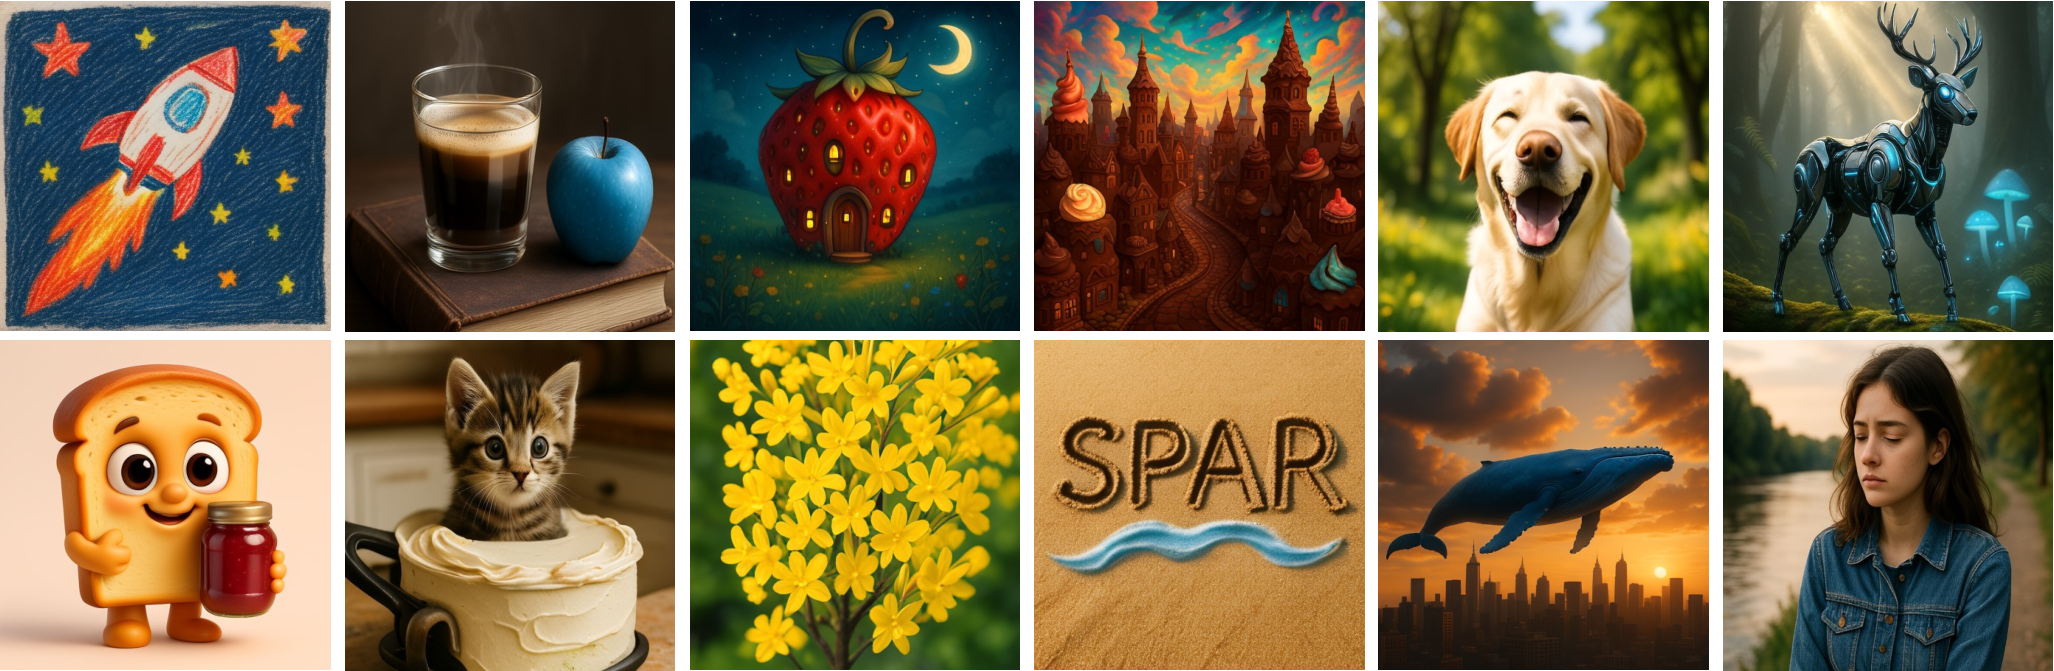
\includegraphics[width=1.\columnwidth]{./images/vis_gen.pdf}
    \vspace{-15pt}
    \caption{Qualitative results of image generation.}
    \label{fig:vis gen}
\end{figure}

\noindent\textbf{Image Generation.}
Table~\ref{tab:geneval_wise} reports the text-to-image generation results on the GenEval~\cite{ghosh2023geneval} and WISE~\cite{niu2025wise} benchmarks, and Figure~\ref{fig:vis gen} illustrates the qualitative results of our method.
We compare SPAR with two categories of methods: generation-only models and unified models that support both understanding and generation. SPAR-3B achieves an overall score of 0.91 on GenEval, ranking first among all compared methods, with the best scores of 0.84 in Counting and 0.87 in Position. Notably, as a unified model, SPAR surpasses even the much larger generation-only model, demonstrating that SPAR's representation space effectively accommodates both understanding and generation without performance degradation. On the knowledge-intensive WISE benchmark, SPAR-3B attains an overall score of 0.64, outperforming all compared methods, further validating that the rich semantic information preserved by the SPAR tokenizer benefits generation quality.
% Moreover, SPAR-1B achieves overall scores of 0.89 (GenEval) and 0.57 (WISE) with only 1B parameter, surpassing many models with substantially larger parameter counts.

\noindent\textbf{Image Editing.}
We evaluate image editing capabilities on ImgEdit-Bench as shown in Table~\ref{tab:imgedit}. SPAR-3B achieves an overall score of 4.01, the highest among all open-source methods, closely approaching the proprietary GPT-4o (4.20). Compared with the second-best OmniGen2 (3.44), SPAR-3B yields an absolute improvement of +0.58.
Across specific editing categories, SPAR-3B achieves the best performance on various subtypes, with particularly pronounced advantages on semantically demanding tasks, indicating that the rich semantic representations within the SPAR tokenizer effectively enhance the editing model's ability to precisely comprehend and execute editing instructions.




\begin{table}[t]
\small
\centering
\caption{{Evaluation of image editing ability on ImgEdit benchmark.} }
\vspace{-10pt}
\begin{tabular}{lcccccccccc}
\toprule
\textbf{Model} & \textbf{Add} & \textbf{Adj.} & \textbf{Ext.} & \textbf{Repl.} & \textbf{Rmv.} & \textbf{Bkg.} & \textbf{Style} & \textbf{Hyb.} & \textbf{Act.} & \textbf{Overall} \\
\midrule
GPT-4o~\cite{openai2025introducing4o} & 4.61 & 4.33 & 2.9 & 4.35 & 3.66 & 4.57 & 4.93 & 3.96 & 4.89 & 4.20 \\
\midrule
MagicBrush~\cite{zhang2023magicbrush} & 2.84 & 1.58 & 1.51 & 1.97 & 1.58 & 1.75 & 2.38 & 1.62 & 1.22 & 1.90 \\
Instruct-P2P~\cite{brooks2023instructpix2pix} & 2.45 & 1.83 & 1.44 & 2.01 & 1.50 & 1.44 & 3.55 & 1.20 & 1.46 & 1.88 \\
AnyEdit~\cite{yu2025anyedit} & 3.18 & 2.95 & 1.88 & 2.47 & 2.23 & 2.24 & 2.85 & 1.56 & 2.65 & 2.45 \\
UltraEdit~\cite{zhao2024ultraedit} & 3.44 & 2.81 & 2.13 & 2.96 & 1.45 & 2.83 & 3.76 & 1.91 & 2.98 & 2.70 \\
OmniGen~\cite{xiao2025omnigen} & 3.47 & 3.04 & 1.71 & 2.94 & 2.43 & 3.21 & 4.19 & 2.24 & 3.38 & 2.96 \\
Step1X-Edit~\cite{liu2025step1x} & 3.88 & 3.14 & 1.76 & 3.40 & 2.41 & 3.16 & 4.63 & 2.64 & 2.52 & 3.06 \\
ICEdit~\cite{zhang2025enabling} & 3.58 & 3.39 & 1.73 & 3.15 & 2.93 & 3.08 & 3.84 & 2.04 & 3.68 & 3.05 \\
BAGEL~\cite{deng2025bagel} & 3.56 & 3.31 & 1.70 & 3.30 & 2.62 & 3.24 & 4.49 & 2.38 & 4.17 & 3.20 \\
UniWorld-V1~\cite{lin2025uniworld} & 3.82 & 3.64 & 2.27 & 3.47 & 3.24 & 2.99 & 4.21 & 2.96 & 2.74 & 3.26 \\
% Janus-4o & 3.60 & 3.25 & 2.28 & 3.27 & 2.28 & 3.32 & 4.47 & 2.74 & 4.13 & 3.26 \\
OmniGen2~\cite{wu2025omnigen2} & 3.57 & 3.06 & 1.77 & 3.74 & 3.20 & 3.57 & 4.81 & 2.52 & {4.68} & 3.44 \\
\rowcolor[HTML]{EFEFEF} \textbf{SPAR-3B} & \textbf{4.31} & \textbf{3.93} & \textbf{2.32} & \textbf{4.52} & \textbf{4.15} & \textbf{4.20} & \textbf{4.87} & \textbf{3.12} & \textbf{4.69} & \textbf{4.01} \\
\bottomrule
\end{tabular}
\label{tab:imgedit}
\end{table}




\subsection{Ablation Studies}

\noindent\textbf{Unified Tokenizer.}
Table~\ref{tab:abl_arch} investigates the contribution of each component in the unified tokenizer. Removing the pixel stream (Row b) leads to a clear reconstruction degradation (PSNR drops by 2.03, SSIM by 0.068), while the understanding metrics remain nearly unchanged, confirming that the semantic encoder alone cannot recover sufficient pixel-level details and the pixel stream is essential for bridging this gap. Removing the semantic stream (Row c) yields better reconstruction than Row~b, yet causes a catastrophic collapse in understanding (MMB drops from 73.0 to 18.4, MME-P from 1500 to 709), demonstrating that without the lightweight semantic anchor, end-to-end pixel-oriented optimization destroys the encoder's discriminative structure. The contrast between Rows~b and c validates the asymmetric design: the semantic stream preserves understanding at minimal cost, while the heavier pixel stream shoulders the reconstruction burden. Finally, freezing the encoder throughout training (Row d) preserves understanding well but results in severely degraded reconstruction (rFID 6.14, PSNR 16.26), verifying that Stage~III encoder fine-tuning with semantic self-distillation is critical for endowing the encoder with pixel representation capability.



\noindent\textbf{Unified Model.}
Table~\ref{tab:abl_dtr} evaluates the two key components of the unified model. Replacing DTR with last-layer-only extraction (Row b) causes the largest overall drop, indicating that adaptively aggregating multi-layer MLLM features provides richer structural and semantic cues than relying solely on the top-layer representation. Removing the self-alignment loss $\mathcal{L}_{\text{align}}$ (Row c) also degrades all three metrics, confirming that leveraging the dual-stream tokenizer as an alignment teacher effectively transfers the accumulated semantic-pixel knowledge to the DiT and improves generation quality without any external feature network.


\begin{table}[t]
\small
\centering
\caption{Ablation on unified tokenizer. Evaluated on ImageNet 50k ($256 \times 256$) for reconstruction and multimodal benchmarks for understanding.}
\vspace{-10pt}
\begin{tabular}{clcccccc}
\toprule
\multirow{2}{*}{\textbf{Row}} & \multirow{2}{*}{\textbf{Setting}} & \multicolumn{3}{c}{\textbf{Reconstruction}} & \multicolumn{3}{c}{\textbf{Understanding}} \\
& & \textbf{rFID}$\downarrow$ & \textbf{PSNR}$\uparrow$ & \textbf{SSIM}$\uparrow$ & \textbf{MME-P} & \textbf{MMB} & \textbf{MMVP} \\ \midrule
(a) & Full Model & \textbf{0.27} & \textbf{26.65} & \textbf{0.856} & \textbf{1500} & \textbf{73.0} & \textbf{68.9} \\
(b) & w/o Pixel Stream & 0.31 & 24.62 & 0.788 & 1499 & 72.6 & 68.7 \\
(c) & w/o Semantic Stream & 0.29 & 25.28 & 0.804 & 709 & 18.4 & 50.0 \\
(d) & Frozen Encoder & 6.14 & 16.26 & 0.572 & 1492 & 72.6 & 67.3 \\
\bottomrule
\end{tabular}
\label{tab:abl_arch}
\end{table}

\begin{table}[t]
\small
\centering
\caption{Ablation on unified model training.}
\vspace{-10pt}
\begin{tabular}{clccc}
\toprule
\textbf{Row} & \textbf{Setting} & \textbf{GenEval}$\uparrow$ & \textbf{WISE}$\uparrow$ & \textbf{ImgEdit}$\uparrow$ \\ \midrule
(a) & Full Model & \textbf{0.89} & \textbf{0.57} & \textbf{3.85} \\
(b) & w/o DTR & 0.86 & 0.54 & 3.73 \\
(c) & w/o Self-Alignment $\mathcal{L}_{\text{align}}$ & 0.86 & 0.53 & 3.78 \\
\bottomrule
\end{tabular}
\label{tab:abl_dtr}
\end{table}


% \section{Conclusion}
% We presented SPAR, a unified multimodal framework that addresses the persistent dichotomy between semantic perception and pixel-level generation. By migrating the generative modeling space from conventional VAE latent spaces to a semantic representation space, SPAR establishes a fully unified paradigm. This is achieved through three key innovations: an asymmetric dual-stream tokenizer that explicitly decouples semantic preservation from pixel reconstruction, dynamic token routing for adaptive multi-layer feature fusion, and a self-aligned generation paradigm that eliminates the reliance on external feature networks. Extensive experiments demonstrate that SPAR sets a new state-of-the-art across diverse benchmarks—including image reconstruction, multimodal understanding, text-to-image synthesis, and complex image editing. Most importantly, SPAR proves that well-structured semantic spaces can serve as a highly effective and robust foundation for building next-generation unified vision-language models without sacrificing the discriminative capabilities of pre-trained encoders.

% \section{Conclusion}
% In this paper, we presented SPAR, a unified multimodal framework that fundamentally resolves the inherent tension between semantic perception and pixel-level generation. Rather than forcing a compromise within a single latent space or relying on external teachers, SPAR demonstrates that these competing objectives can be elegantly harmonized. By introducing an asymmetric dual-stream tokenizer, we explicitly decouple semantic preservation from fine-grained pixel reconstruction. Coupled with dynamic token routing to adaptively satisfy the hierarchical feature demands of varying tokens, and a self-alignment paradigm, SPAR effectively eliminates the rigidities of previous unified models. Comprehensive evaluations across image reconstruction, multimodal understanding, generation, and complex editing tasks confirm that our approach achieves state-of-the-art performance.
% Ultimately, this work provides a compelling blueprint for the community: natively aligned, well-structured semantic spaces can indeed serve as a robust and uncompromising foundation for the next generation of unified vision-language models.
\section{Conclusion}
In this paper, we presented SPAR, a unified multimodal framework that addresses the fundamental feature discrepancy between semantic perception and pixel-level generation. To overcome the detail loss inherent in semantic spaces, we introduced an asymmetric dual-stream tokenizer that explicitly decouples semantic preservation from high-quality pixel reconstruction. Furthermore, we proposed dynamic token routing to adaptively harness multi-layer MLLM representations, along with a self- lignment paradigm that eliminates the reliance on external representation teachers. Extensive experiments demonstrate that SPAR achieves state-of-the-art performance across diverse benchmarks, delivering high-fidelity image generation and complex editing without degrading the pre-trained understanding capabilities.
% 

% \section*{Acknowledgements}
% Please insert your acknowledgments here.

% ---- Bibliography ----
%
% BibTeX users should specify bibliography style 'splncs04'.
% References will then be sorted and formatted in the correct style.
%
\bibliographystyle{splncs04}
\bibliography{main}
\end{document}
